\section{Results}
\label{sec:result}



\begin{figure*}[ht]
\centering     %%% not \center
\subfigure[Random]{\label{fig:a}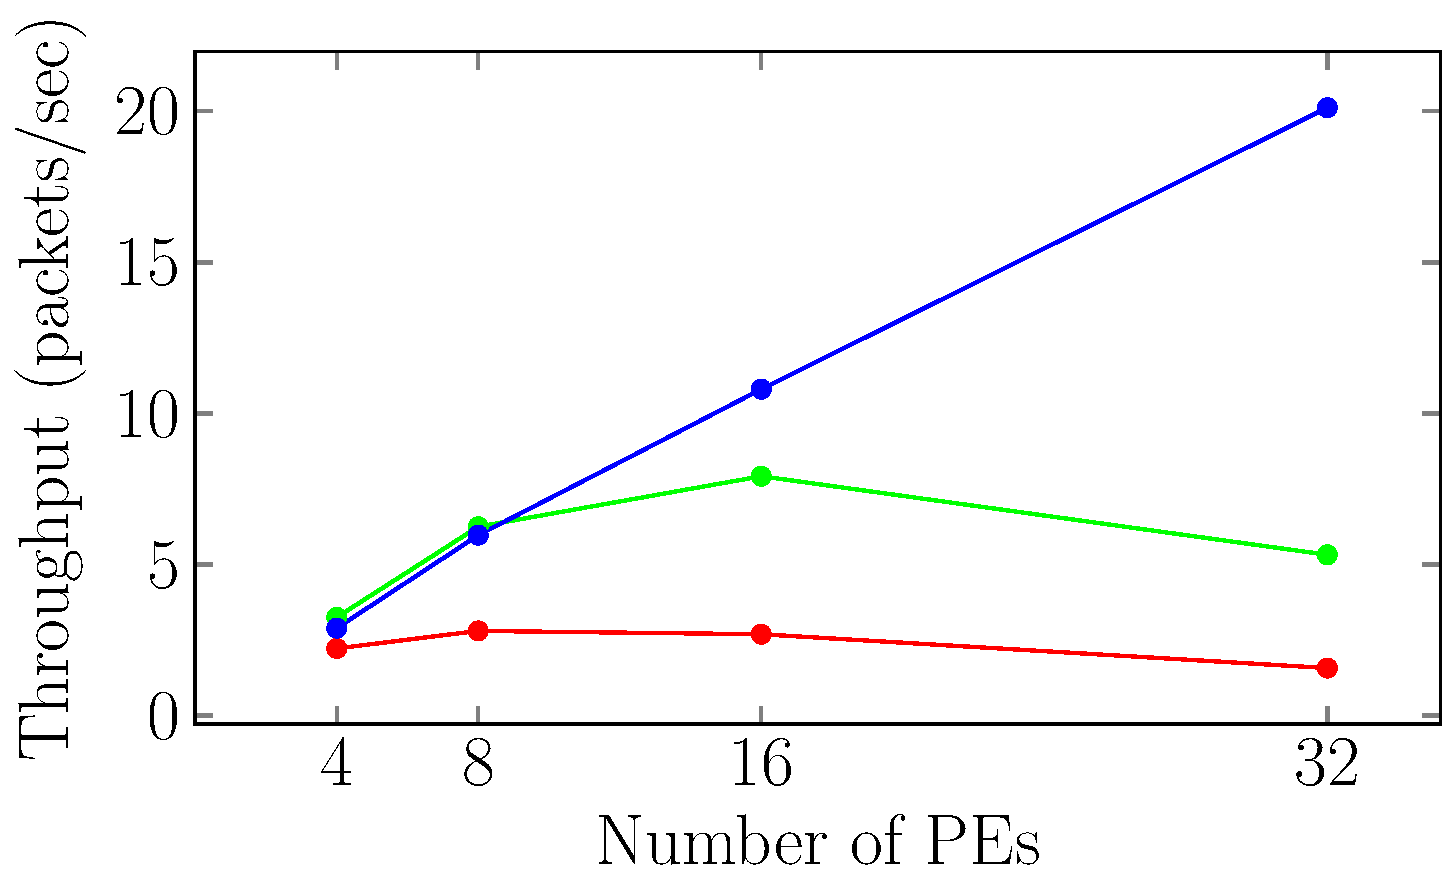
\includegraphics[width=0.5\columnwidth]{Data/randomTput.pdf}}
\subfigure[Tornado]{\label{fig:b}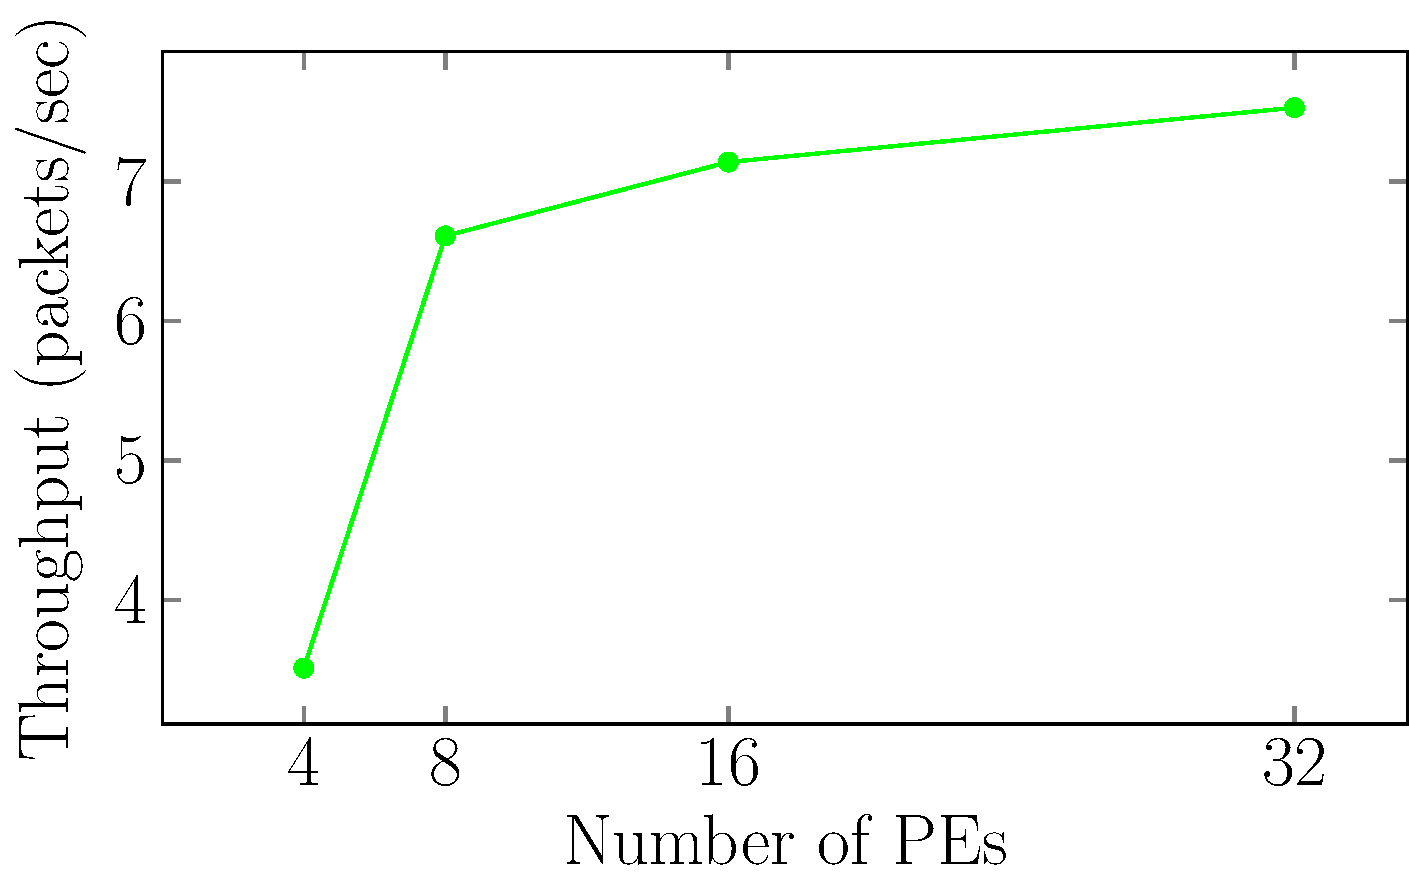
\includegraphics[width=0.5\columnwidth]{Data/tornadoTput.pdf}}
\subfigure[Complement]{\label{fig:a}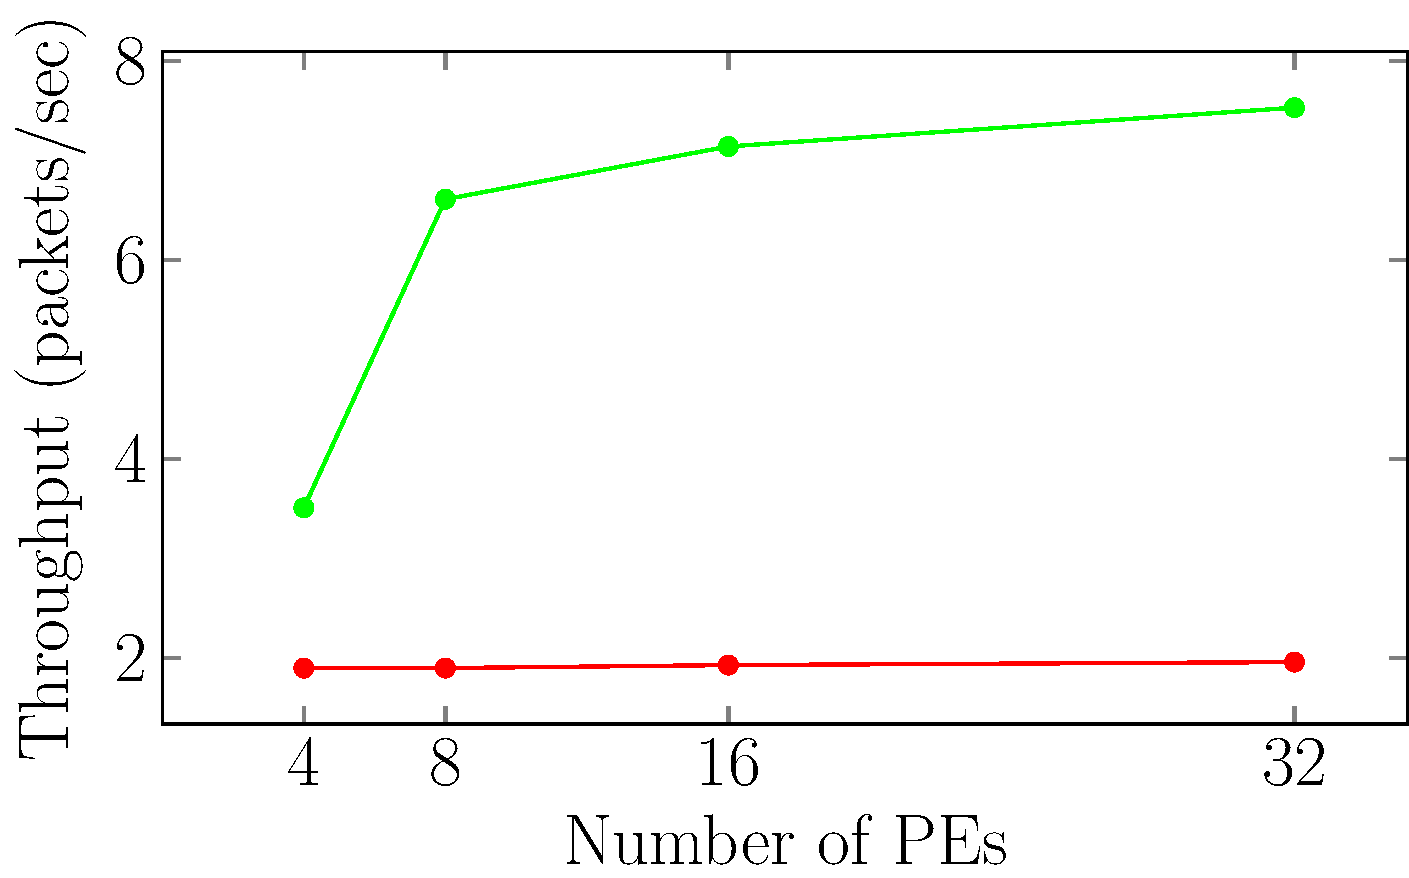
\includegraphics[width=0.5\columnwidth]{Data/complementTput.pdf}}
\subfigure[Reverse]{\label{fig:b}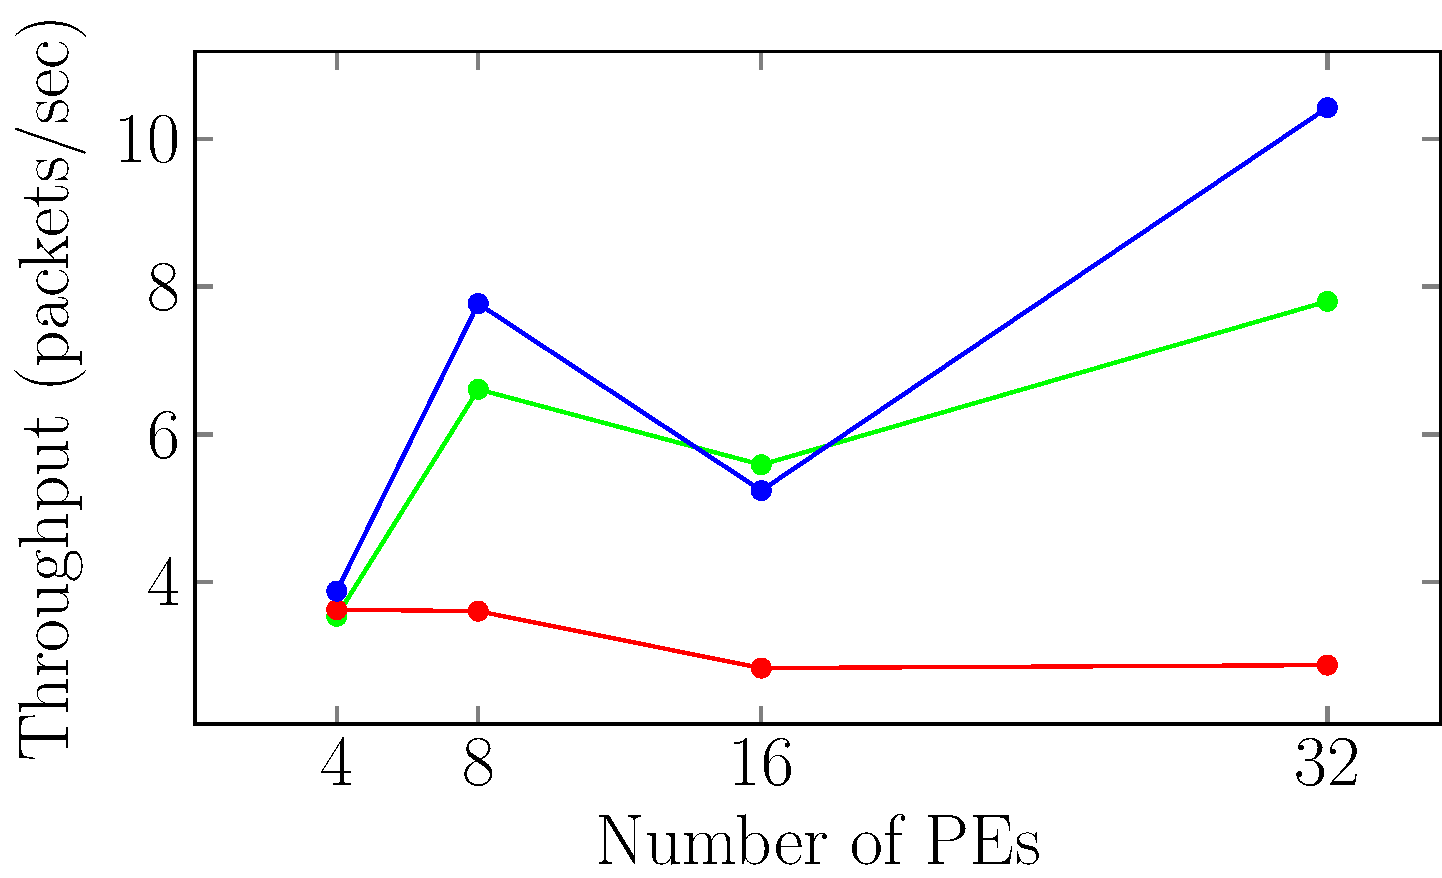
\includegraphics[width=0.5\columnwidth]{Data/reverseTput.pdf}}
\caption{Throughput of different Binary Noc architectures with varying size corresponding to different traffic patterns}
\end{figure*}

\begin{figure*}[ht]
\centering     %%% not \center
\subfigure[Figure A]{\label{fig:a}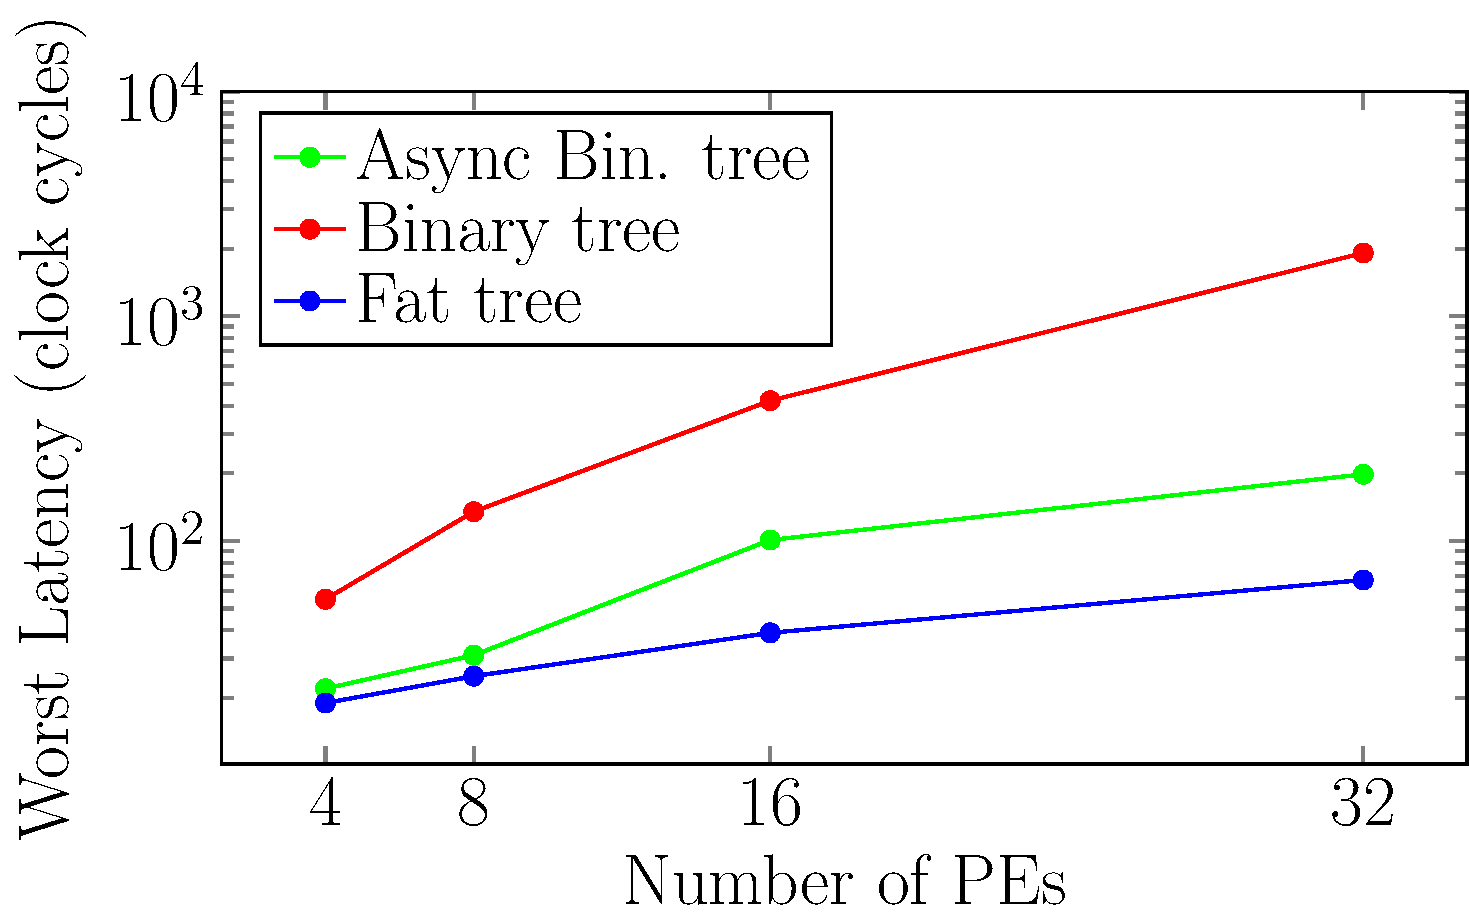
\includegraphics[width=0.5\columnwidth]{Data/randomLatency.pdf}}
\subfigure[Figure B]{\label{fig:b}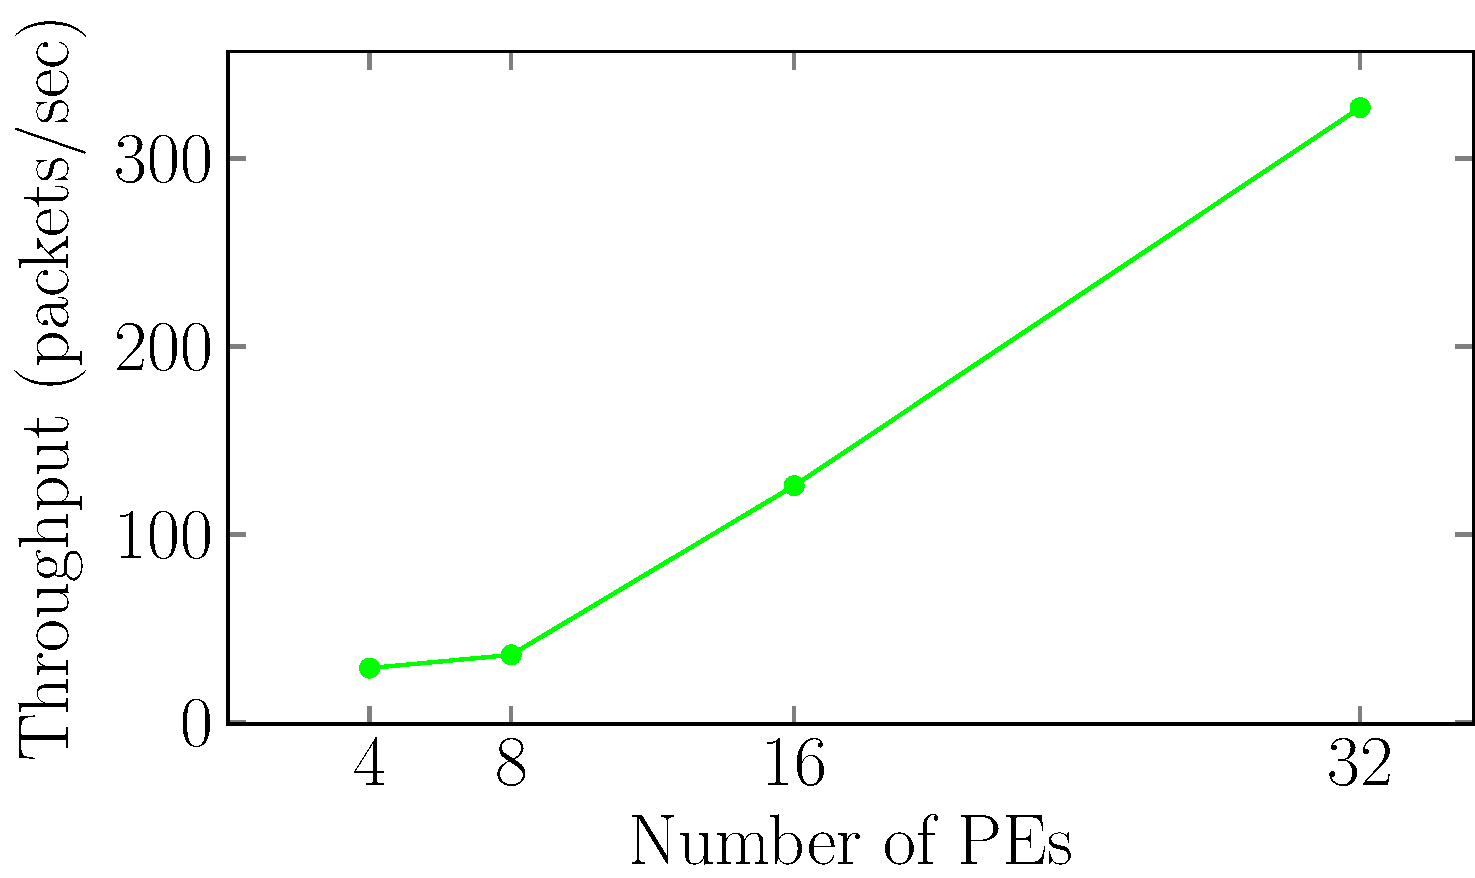
\includegraphics[width=0.5\columnwidth]{Data/tornadoLatency.pdf}}
\subfigure[Figure A]{\label{fig:a}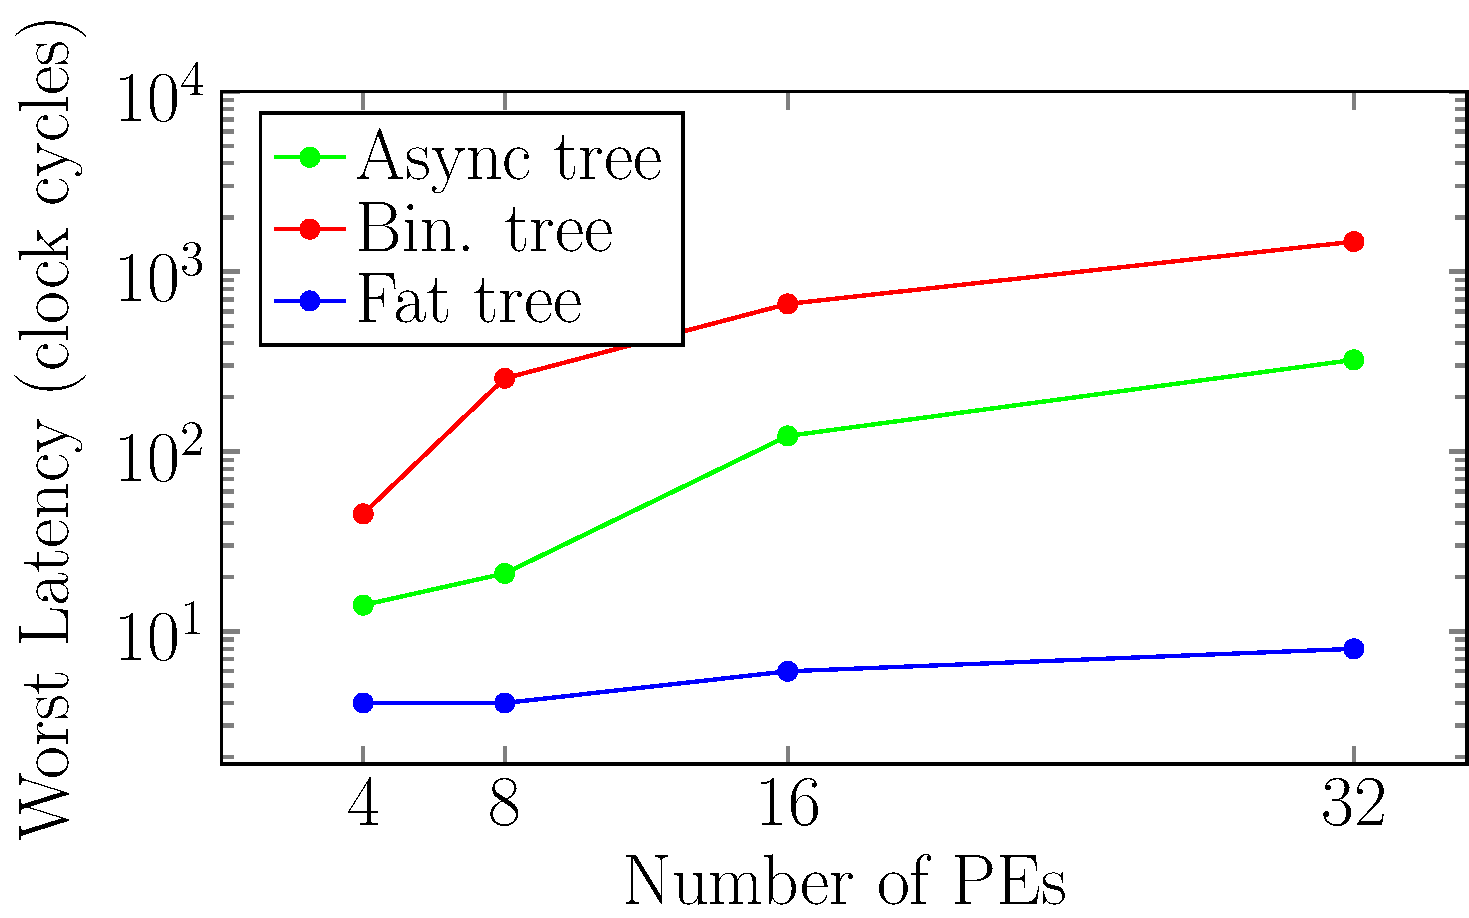
\includegraphics[width=0.5\columnwidth]{Data/complementLatency.pdf}}
\subfigure[Figure B]{\label{fig:b}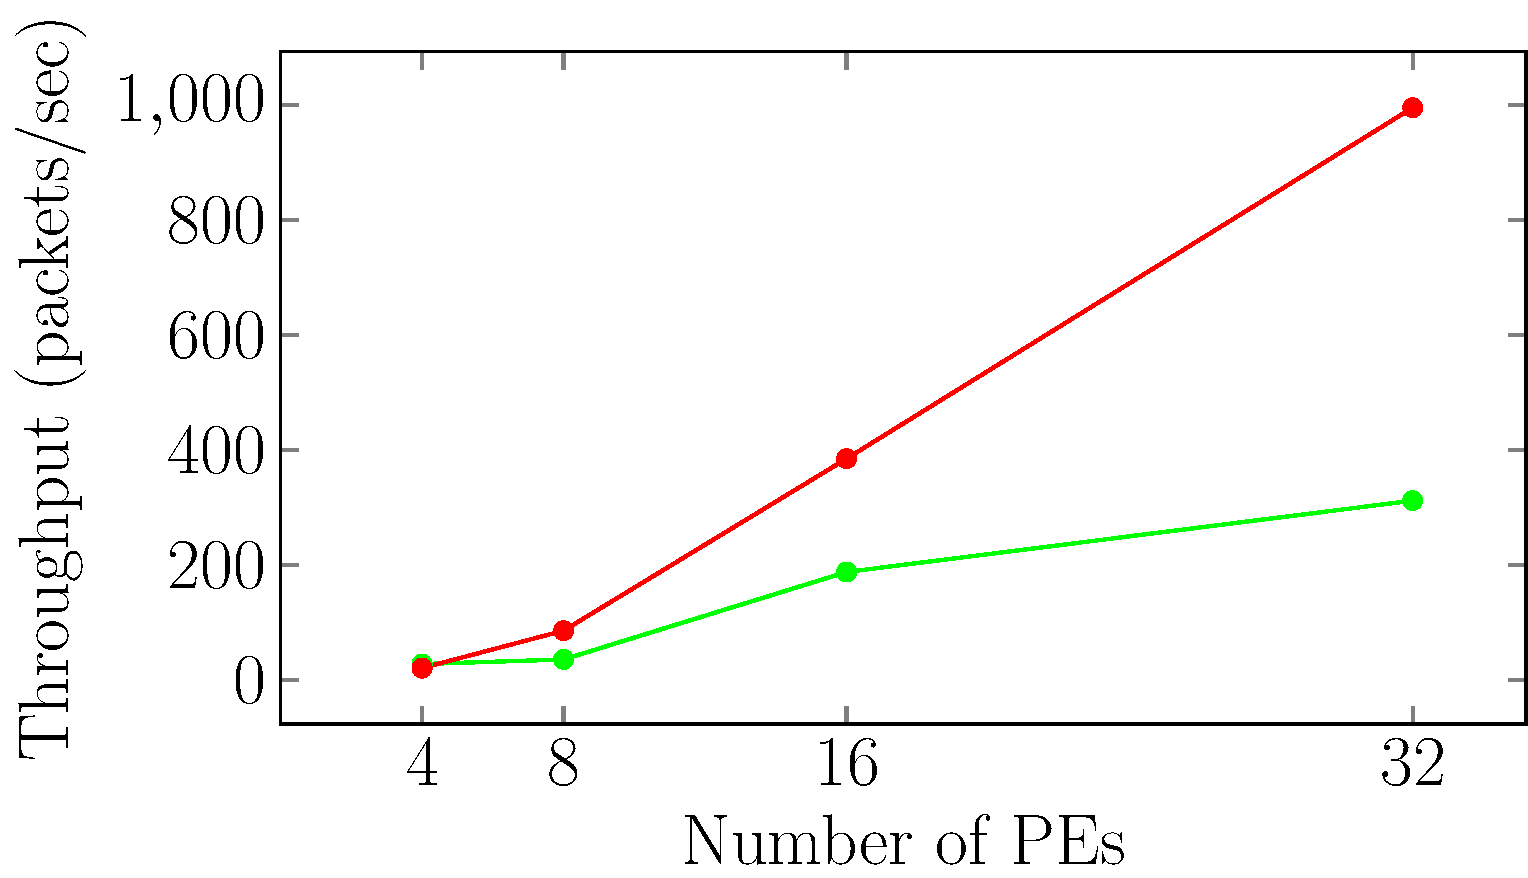
\includegraphics[width=0.5\columnwidth]{Data/reverseLatency.pdf}}
\caption{Maximum latency of different Binary Noc architectures with varying size corresponding to different traffic patterns}
\end{figure*}

Table~\ref{table:systemResourceConsumption} compares the resource utilization and the maximum frequency of operation for HNoC and CONNECT for different number of PEs
\input Tables/SystemResource


